\documentclass[12pt,a4paper]{article}


\usepackage{macros}

\begin{document}\thispagestyle{empty}

\centerline{\Large \bf Homework 4: Due at class on March 26}
 \vspace{.5cm}

The Einstein summation convention is applied in all the given problems.



 \vspace{.5cm}
 \noindent \textbf{1}. 
 Let us consider the following action
\begin{equation}
S=\int_a^b d t \left({g_{i j} \frac{d x^i}{d t} \frac{d x^j}{d t}}\right)
\end{equation}
The equation of motion minimizes the action, namely $\delta S=0$ under the variation $\tilde x(t)=x(t)+\delta x(t)$ where we fix the initial and final condition $x(a)=x_i$, $x(b)=x_f$. Show that the equation of motion is equivalent to the geodesic equation. 
 
 
 \vspace{.5cm}
 \noindent \textbf{2}.  Derive the expression of the Christoffel symbols
$$
\Gamma_{i j}^k=\frac{1}{2}\left(\frac{\partial g_{j l}}{\partial x^i}+\frac{\partial g_{i l}}{\partial x^j}-\frac{\partial g_{i j}}{\partial x^l}\right) g^{l k}
$$
from
$$
\frac{\partial}{\partial x^i} g_{j k}=g\left(\nabla_{\frac{\partial}{\partial x^i}} \frac{\partial}{\partial x^j}, \frac{\partial}{\partial x^k}\right)+g\left(\frac{\partial}{\partial x^j}, \nabla_{\frac{\partial}{\partial x^i}} \frac{\partial}{\partial x^k}\right)
$$
and its permutations with respect to $i, j, k$. Show that the Riemann curvature can be written
$$
R^l{}_{i j k}=\Gamma_{j k}^s \Gamma_{i s}^l-\Gamma_{i k}^s \Gamma_{j s}^l+\frac{\partial \Gamma_{j k}^l}{\partial x^i}-\frac{\partial \Gamma_{i k}^l}{\partial x^j} 
$$
in terms of local coordinates.



 \vspace{.5cm}
 \noindent \textbf{3}. 
A vector field $X$ is a Killing field if the Lie derivative with respect to $X$ of the metric $g$ vanishes:
$$
{L}_X g=0~.
$$
Show that this is equivalent to 
$$
g\left(\nabla_Y X, Z\right)+g\left(Y, \nabla_Z X\right)=0
$$
for all vectors $Y$ and $Z$ where $\nabla$ is  the Levi-Civita connection. In terms of local coordinates where $X=X^j\partial_j$, show that this amounts to 
$$
\nabla_{\partial_i} X_j+\nabla_{\partial_j} X_i=0~.
$$
Also, show that this is equivalent to
\begin{equation}
X^k \partial_k g_{i j}+g_{k j} \partial_i X^k+g_{i k} \partial_j X^k=0
\end{equation}

 \vspace{.5cm}
 \noindent \textbf{4}. Let $\iota:S^2 \hookrightarrow \bR^3$ be the inclusion of the 2-sphere with unit radius.  Let $g:ds^2=\sum_{i=0}^2dx^i\otimes dx^i$ be the standard metric of $\bR^3$. Find the induced metric $\iota^* g$ on $S^2$ in terms of the polar coordinate of $\bR^3$.
\begin{align}
x^0&=r\sin\theta \cos\phi\cr
x^1&=r\sin\theta \sin\phi\cr
x^2&=r\cos\theta\nonumber
\end{align}
Given this metric, find geodesics on $S^2$ and compute its Riemann, Ricci and scalar curvature.

 Do parallel transport of a vector along a triangle $\Delta$PQR on a unit sphere (Figure 1) with respect to the Levi-Civita connection of the metric and find the angle difference when it comes back.  Compare it with the area of the triangle (see Homework 1).


 \begin{figure}[h]\centering
  \includegraphics[width=5cm]{triangle}
 \caption{A triangle on a 2-sphere}
 \end{figure}

%\vspace{.5cm}
%\noindent  \textbf{2}. Let $ds^2=-dt^2+dx^2+dy^2$ be the Minkowski metric on $\bR^{1,2}$ and $-t^2+x^2+y^2=-1$ for $t>0$ be the space-like surface (hyperboloid $\mathbf{S}$). (See Figure 1.) Find the induced metric on the hyperboloid $\mathbf{S}$ in terms of the polar coordinate
%\begin{align}
%t&=r \cosh \rho  \cr
%x&=r\sinh\rho\cos\phi\cr
%y&=r\sinh\rho \sin\phi\nonumber
%\end{align}
%Given this metric, find geodesics on $\mathbf{S}$ and compute its Riemann, Ricci and scalar curvature.




%\vspace{.5cm}
%\noindent  \textbf{3}. Let us consider the unit disk $\mathbf{D}$ on the x-y plane. Let $\pi(P)$ be the intersection point of the unit disk and the line between the  point $(0,0,-1)$ and $P\in \mathbf{S}$. By assigning $\pi(P)$ to $P$, there is one-to-one map from the unit disk $D$ and the hyperboloid $\mathbf{S}$.
%Show that the map $\pi^{-1}:\mathbf{D}\to \mathbf{S}$ is determined by
%$$
%(u,v) \mapsto \left(\frac{2u}{1-u^2-v^2},\frac{2v}{1-u^2-v^2},\frac{1+u^2+v^2}{1-u^2-v^2} \right)~.
%$$
%Find the metric on the unit disk pull-backed by this map. The unit disk $\mathbf{D}$ with this induced metric is called the Poincar\'e disk.
%
%The red curve on the hyperboloid is an intersection with a plane (pink in Figure 2,3) that goes through the origin. We put a disk (called Klein's disk) on the bottom of the hyperboloid, which allows us to get the corresponding straight line (green) on Klein's disk. This curve is mapped by $\pi:\mathbf{S}\to \mathbf{D}$ to an (red) arc in the Poincare disk. If the green line is represented by $x=a$ (Figure 4), find the equation for the red curve.
%
%Find geodesics on $\mathbf{D}$ and compute its Riemann, Ricci and scalar curvature.

%
% \vspace{.5cm}
% \noindent 6. We consider the unite 2-sphere $S^2\subset \bR^3$ with metric induced from $\bR^3$ as in problem 2. Let us define a smooth map $f:S^2\to \bR$ by $f(x^0,x^1,x^2)=x^2$. Then, explicitly write the gradient vector of $f$ and its flow $\varphi_t$.



%
%
%
%\begin{figure}[h]
%  \begin{minipage}[b]{8cm}\centering
% \includegraphics[width=8cm]{hyperboloid}
%\caption{Hyperboloid and Poincare disk}
%\end{minipage}
%  \begin{minipage}[b]{8cm}\centering
% \includegraphics[width=6.5cm]{hyperboloid2}
% \caption{Hyperboloid and Poincare disk}
%\end{minipage}
%\end{figure}
%
%\begin{figure}[h]\centering
% 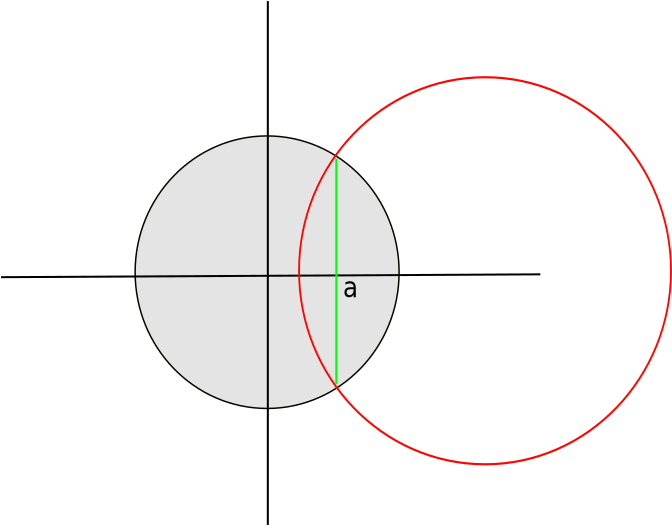
\includegraphics[width=5cm]{disk}
%\caption{Poincare disk}
%\end{figure}
%



\end{document}
